% !TEX output_directory=output
\documentclass{beamer}

\usepackage[beamer]{kaufman}

\bibliography{../refs.bib}
\graphicspath{{../graphics/}}

\title{Hamiltonian Engineering via Reinforcement Learning}
\author{Will Kaufman}
\institute{Ramanathan Group \\ Dartmouth College}

\titlegraphic{\includegraphics[height=.1\textheight]{LonePine.pdf}}

\begin{document}

\frame{\titlepage}

\begin{frame}
\frametitle{Table of Contents}
\tableofcontents
\end{frame}

\section{Hamiltonian engineering}

\begin{frame}
\frametitle{Hamiltonian engineering}

Hamiltonian engineering seeks to control the system's evolution so that it appears to evolve under a target ``effective'' Hamiltonian.

\begin{equation}
    H(t) = H_\text{system} + H_\text{control}(t)
\end{equation}

\begin{equation}\label{eq:strob_measure}
    \rho(Nt_c) = U_\text{target}(Nt_c) \rho(0) U_\text{target}^\dagger(Nt_c)
\end{equation}

\pause

In NMR \cite{1976ii}\dots

\begin{align}\label{eq:ham_spin}
    H_\text{system} &= \sum_i \delta_i I_z^i + \sum_{i,j} d_{ij} \left( 3I_z^iI_z^j - \mathbf{I^i} \cdot \mathbf{I^j} \right)
    = H_\text{CS} + H_\text{D} \\
    H_\text{control}(t) &= -B_1(t) \sum_i \gamma_n^i I_x^i
\end{align}

\end{frame}

\section{Previous approaches}

\begin{frame}
\frametitle{Average Hamiltonian theory}

TODO continue here...

\end{frame}

\begin{frame}
\frametitle{Average Hamiltonian theory: benefits and limitations}



\end{frame}

\begin{frame}
\frametitle{GRAPE}

Text

\end{frame}

% TODO add benefits/limitations of?

\section{Reinforcement learning as alternative approach}

\begin{frame}
\frametitle{Reinforcement learning paradigm}

% TODO intro section to RL, relate to MDP?

\begin{figure}
    \centering
    \scalebox{.5}{
    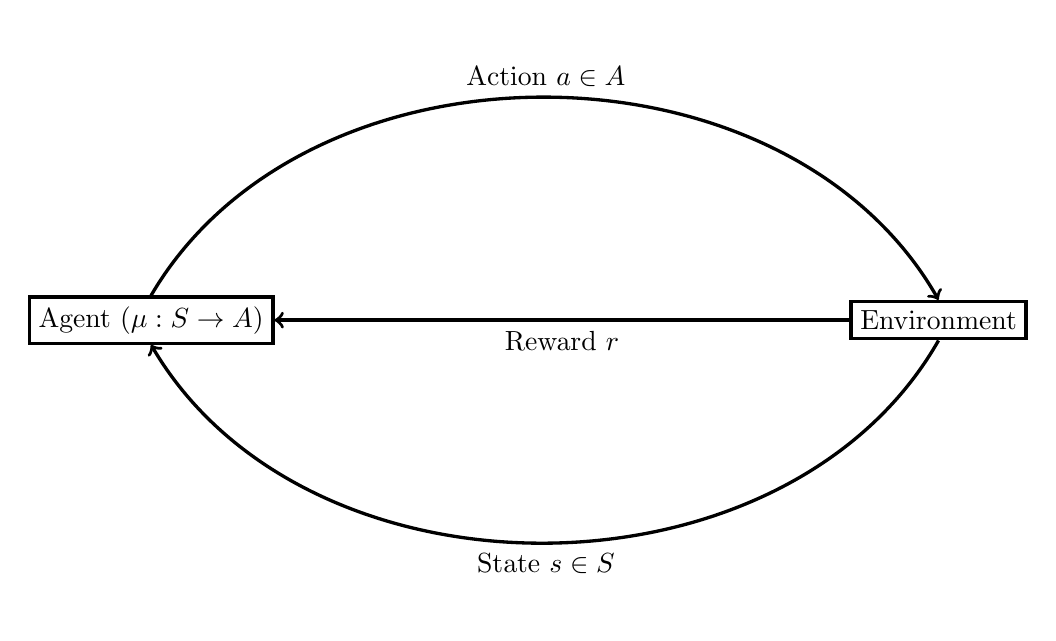
\begin{tikzpicture}[->, very thick]
         %nodes
         \node[draw] at (-5,0) (agent) {Agent ($\mu: S \to A$)};
         \node[draw] at (5,0) (env) {Environment};
         \path
             (agent.north) edge[bend left=60] node[above] {Action $a \in A$} (env.north)
             (env.south) edge[bend left=60] node[below] {State $s \in S$} (agent.south)
             (env.west) edge node[below] {Reward $r$} (agent.east);
    \end{tikzpicture}
    }
    %\caption{The general reinforcement learning paradigm.}
    \label{fig:RL}
\end{figure}

\end{frame}

\begin{frame}
\frametitle{RL Definitions}

% TODO define S, A, pi, V or Q

\end{frame}

\begin{frame}
\frametitle{Actor-critic methods}

% TODO include Bellman equation, gradient update rules

\end{frame}

\begin{frame}
\frametitle{Evolutionary reinforcement learning}

% TODO diagram

\end{frame}

\begin{frame}
\frametitle{Applying RL to Hamiltonian engineering}

% TODO make a table?
%How things relate

\end{frame}

\section{Results}

\begin{frame}
\frametitle{Hyperparameter search and algorithm performance}
% TODO
\end{frame}

\begin{frame}
\frametitle{Hyperparameter search and algorithm performance (cont.)}
% TODO
\end{frame}

\begin{frame}
\frametitle{Candidate pulse sequences}

% TODO
% general evaluation strategy (compare to WHH-4, MREV-8)
% compare on similar timeframe
% robustness?
% simulation parameters

\end{frame}

\begin{frame}
\frametitle{Candidate pulse sequences (cont.)}
% TODO
\end{frame}

\section{Next steps}

\begin{frame}
\frametitle{Improvements to RL algorithm}
% TODO
% convergence, speed, robustness, efficiency
% change setup to GRAPE-like tests (likely won't be as effective)
\end{frame}

\begin{frame}
\frametitle{Experimental verification of candidate pulse sequences}
% TODO
\end{frame}

\begin{frame}
\frametitle{Bibliography}

\printbibliography

\end{frame}






\end{document}
